\chapter{Overzicht van de testomgeving}
\label{sec:environment}

De testomgeving om OpenStack op uit te rollen bestaat uit 3 Ubuntu Server 16.04.02 LTS systemen met elk 8 GB vRAM, 2 vCPU's met 4 kernen en 10 GB HDD opslag. Deze 3 systemen worden gevirtualiseerd met behulp van VMWare ESXI 5.5 update 2 op 1 fysieke server. Via drie SSH-verbindingen kunnen de systemen aangestuurd worden. Figuur~\ref{fig:environment} geeft een schematisch overzicht weer van de drie systemen.

De OpenStack-omgeving bestaat uit 1 controller node en 2 compute nodes. De node \textit{jerico-03} doet dienst als controller node waarbij alle nodige services van OpenStack zijn geactiveerd. De nodes jerico-02 en jerico-03 doen dienst als compute-nodes en enkel de hiervoor nodige services zijn geactiveerd. Een overzicht van de actieve services per node bevindt zich in Tabel~\ref{tab:test_environment}. Een overzicht van alle services met bijhorende uitleg bevinden zich in \hyperref[att:openstack_services]{Bijlage B}.

\begin{table}[tbp]
  \centering
  \caption{Overzicht van de actieve services per node}
  \label{tab:test_environment}
  \begin{tabular}{cccccccccc}
    \hline
    Host      & KeyStone & Glance & Neutron & Nova & Cinder & Horizon & Heat & Ceilometer & Aodh \\ \hline
    jerico-03 & \checkmark        & \checkmark      & \checkmark       & \checkmark    & \checkmark      & \checkmark       & \checkmark    & \checkmark          & \checkmark    \\
    jerico-02 &          &        & q-agt   & n-cpu  & c-vol    &         &      & \checkmark          & \checkmark    \\
    jerico-01 &          &        & q-agt   & n-cpu  & c-vol    &         &      & \checkmark          & \checkmark    \\ \hline
  \end{tabular}
\end{table}

\begin{figure}
  \centering
  \captionsetup{justification=centering}
  \begin{subfigure}{\textwidth}
    \centering
    \centerline{
      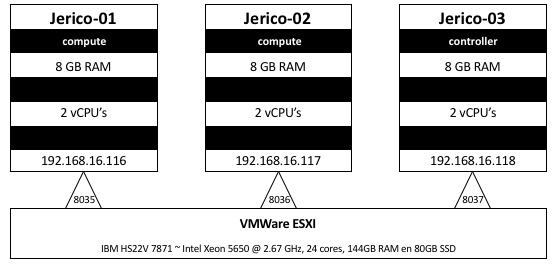
\includegraphics[scale=0.5]{Test_environment}
    }
  \end{subfigure}
  \caption{Overzicht van de testomgeving}
  \label{fig:environment}
\end{figure}

\section{DevStack}

OpenStack kan op verschillende manieren worden uitgerold zoals met Autopilot, conjure-up, alsook via DevStack. DevStack~\cite{OpenStack2017a} is een collectie van \textit{bash scripts} ontwikkeld door de community van OpenStack zelf dat volledig automatisch, mits enkele voorafgaande instellingen, OpenStack met al zijn componenten installeert en configureert. In een \textit{local.conf} bestand kunnen alle instellingen worden gewijzigd zoals de verschillende wachtwoorden, de IP-adressen, welke services actief moeten zijn, etc. Een aangemaakte stack gebruiker met \textit{sudo-}permissies kan het script uitvoeren en zo OpenStack volledig installeren op het desbetreffende systeem. \hyperref[att:installation]{Bijlage A} bevat een stap-voor-stap installatiehandleiding van OpenStack met behulp van DevStack.

Aangezien DevStack nog volop in ontwikkeling is (de huidige versie is 0.0.1\footnote{22 maart 2017}), zijn er een aantal gekende problemen. Het grootste probleem is dat OpenStack niet meer naar behoren zal werken na een heropstart van het systeem met als mogelijke oorzaak het niet opnieuw automatisch initialiseren van de daarvoor gebruikte \textit{screens} van DevStack in Ubuntu. Hierdoor worden bepaalde services niet meer gestart en is de enige mogelijkheid het opnieuw uitvoeren van het \textit{stack.sh} bestand als stack-gebruiker. Hierbij wordt alles gewist, van draaiende instanties in OpenStack tot de volledige databank die OpenStack gebruikt wat in de meeste gevallen leidt tot ongemakken. Een 'echte' oplossing voor dit probleem bestaat nog niet, maar de ontwikkeling hiervan is bezig. Een eventuele optie om dit op te lossen zijn volgende commando's:

\begin{code}
\begin{minted}[breaklines]{bash}
$ sudo su stack
$ sudo chown stack:stack `readlink /proc/self/fd/0`
$ screen -c /devstack/stack-screenrc
\end{minted}
\caption{Heropstart van DevStack na systeemherstart}
\end{code}

Dit zou de screens terug moeten koppelen aan Ubuntu en de services van OpenStack terug starten aan de hand van de services die voor de heropstart aan het draaien waren. Uitgebreide testen of dit al dan niet werkt moeten in de toekomst nog uitgevoerd worden.

Daarnaast gebeuren er bijna dagelijks \textit{commits} met verschillende oplossingen waardoor er hoogstwaarschijnlijk verschillende bugs aanwezig zijn in de gebruikte testomgeving.

\section{Nova scheduler}

OpenStack levert Nova af met een standaard \textit{filter and weighting}-scheduler die zal bepalen op welke host, ook wel \textit{hypervisor} genoemd, de nieuwe instantie geplaatst wordt. Het plaatsingsproces gebeurt in twee stappen. Eerst gaan alle beschikbare hypervisors door verschillende filters om te bepalen of de hypervisor de instantie kan hosten. Voorbeelden van standaard meegeleverde filters zijn de RamFilter, DiskFilter, AllHostFilter, en nog vele anderen. In het configuratiebestand van Nova (standaard \textit{nova.conf in /etc/nova/}) bevindt er zich een lijst met alle filters die gebruikt worden tijdens het verkiezingsproces. Zo zal de RamFilter alleen de hypervisors toelaten die voldoende RAM-geheugen ter beschikking hebben terwijl de AllHostFilter alle hypervisors zal toelaten, ongeacht deze plaats hebben voor de nieuwe instantie of niet. Vervolgens worden de toegelaten instanties gesorteerd volgens een bepaald gewicht waardoor de beste hypervisor de nieuwe instantie mag hosten. Figuur~\ref{fig:filteringWorkflow} geeft dit proces schematisch weer.

\begin{figure}
  \centering
  \captionsetup{justification=centering}
  \begin{subfigure}{\textwidth}
    \centering
    \centerline{
      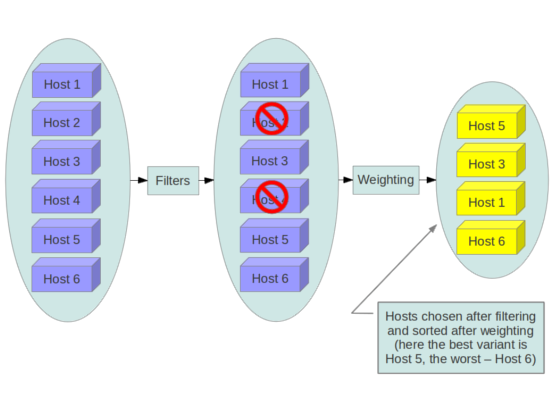
\includegraphics[scale=0.80]{filteringWorkflow1}
    }
  \end{subfigure}
  \caption{Werking van de Nova-scheduler~\cite{OpenStack2017c}}
  \label{fig:filteringWorkflow}
\end{figure}

\subsection{Round Robin scheduler}

Zoals beschreven in~\ref{sec:problem} zal er een proof-of-concept (PoC) worden uitgevoerd om de evaluatie van een resource allocatieschema aan te tonen. Hier is gekozen voor het relatief eenvoudig Round Robin schema, wat een nieuwe instantie steeds op de volgende hypervisor in de rij zal plaatsen. Een hypervisor waarbij net een nieuwe instantie is geplaatst zal zich achteraan in de rij bevinden. Concreet, de eerste instantie zal gehost worden op jerico-01, de tweede op jerico-02, de derde op jerico-03, de vierde op jerico-01 en zo verder.

Aangezien OpenStack en al zijn componenten open-source zijn, biedt het de optie om eigen nova-filters en -weighters te implementeren. Hieraan zijn wel enkele voorwaarden verbonden. Zo moet een custom-filter steeds overerven van \textit{filters} die zich in het \textit{Nova.scheduler}-pakket bevinden (ook wel de \textit{BaseHostFilter} genaamd). Bovendien moet de methode \textit{host\textunderscore passes} geïmplementeerd worden dat de waarde \textit{True} als resultaat teruggeeft indien de hypervisor geschikt is om de instantie te hosten, en \textit{False} indien de hypervisor niet geschikt is voor het hosten van de instantie.

Om het Round Robin algoritme eenvoudig in OpenStack te kunnen implementeren, is hiervoor een \textit{RoundRobinFilter} ontwikkeld. Deze laat enkel de host, die als eerste in de virtuele rij staat, toe om de nieuwe instantie te hosten. De hiervoor gebruikte code bevindt zich hieronder.

\begin{code}
\inputminted{python}{round_robin_filter.py}
\caption{RoundRobinFilter}
\end{code}


Bij iedere nieuwe aanmaak van een instantie zal elke hypervisor door deze filter passeren. Enkel de hypervisor die als eerste in de virtuele rij staat, bepaald door de \textit{counter}, zal True als resultaat van de methode teruggeven en uiteindelijk de nieuwe instantie hosten.

\subsection{Inpluggen van de Round Robin Scheduler}

Om de Round Robin scheduler te activeren in de gebruikte OpenStack omgeving moeten volgende stappen gebeuren:

\begin{enumerate}
  \item Bewaar bovenstaande code in /opt/stack/nova/nova/scheduler/filters/round\textunderscore robin\textunderscore filter.py (naam vrij te kiezen)
  \item Pas het /etc/nova/nova.conf bestand aan zodat in de [DEFAULT]-sectie de lijst van \textit{scheduler\textunderscore default\textunderscore filters} vervangen wordt door \textit{RoundRobinFilter} (naam van de klasse)
  \item Controleer ook in dit bestand of de \textit{scheduler\textunderscore driver} staat ingesteld op \textit{filter\textunderscore scheduler}
  \item Als laatste moet de Nova-scheduler worden herstart. Gebruik hiervoor het commando \textit{\$ screen -x stack} om de screens te betreden, navigeer vervolgens naar het \textit{n-sch} screen en herstart deze service door deze te stoppen (ctrl + c) en terug te starten (pijl naar boven + enter)
\end{enumerate}

Het gebruik van de screens van OpenStack staat uitgelegd in \hyperref[att:installation]{Bijlage A}.

Zoals te zien is in het \textit{nova.conf}-bestand, zijn er verschillende mogelijkheden om de scheduler van Nova te wijzigen. In dit geval is er voor een relatief eenvoudige optie gekozen om een nieuw allocatieschema te gebruiken. Meer complexere allocatieschema's zullen ook aanpassingen van de scheduler\textunderscore driver vereisen voor een correcte werking maar daar wordt niet dieper op ingegaan.

\section{FaaFo - First App Application For OpenStack}
\label{sec:faafo}

Een cloud-applicatie is optimaal indien het de mogelijkheid biedt om te schalen. FaaFo~\cite{OpenStack2017j} is een OpenStack-applicatie die fractalen, voorbeeld in Figuur~\ref{fig:fractal}, van een bepaalde grootte berekent. FaaFo is ontwikkeld door OpenStack om horizontaal uit te schalen. In dit onderzoek is FaaFo uitgerold op minimaal twee nodes. De eerste is de controller-node, die de databank en de queue beheert en de verschillende workers opdrachten kan geven om fractalen te berekenen. De twee node is bijgevolg een worker-node die een fractaal uit de queue van de controller-node zal berekenen en het resultaat zal bewaren in de databank op de controller-node.

De mogelijkheid om te schalen binnen deze applicatie komt door de goede opsplitsing van de verschillende taken in \textit{microservices} en door gebruik te maken van een queue waar de fractalen, die nog berekend moeten worden, in worden bewaard. Een optimaal scenario om te schalen zou als volgt verlopen: indien de enige worker veel CPU-kracht gebruikt binnen een bepaalde periode, dan moet er een tweede worker worden aangemaakt die de eerste worker zal helpen met al het werk. Blijken deze twee samen dan nog veel CPU-kracht te gebruiken, dan wordt een eventuele derde, vierde, ... worker aangemaakt. Indien er meer dan twee workers actief zijn en indien de queue leeg is, dan moeten de overbodige workers worden verwijderd. Dit hele proces wordt eveneens verduidelijkt in Figuur~\ref{fig:flow_chart}.

\begin{figure}
  \centering
  \captionsetup{justification=centering}
  \begin{subfigure}{\textwidth}
    \centering
    \centerline{
      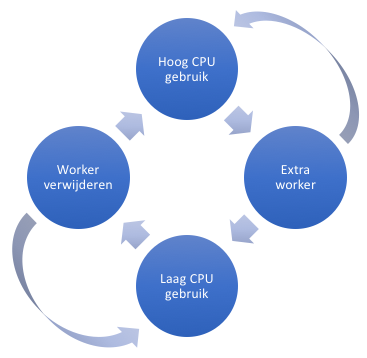
\includegraphics[scale=0.50]{flow_chart}
    }
  \end{subfigure}
  \caption{FaaFo: het schaalscenario}
  \label{fig:flow_chart}
\end{figure}

Het scenario is sterk gerelateerd aan de werkelijke gang van zaken binnen cloud computing. Zoals beschreven in Sectie~\ref{sec:what_is_cloud_computing} en in Sectie~\ref{sec:rmcloud} moet een cloud-gebruiker enerzijds schalen zodat de SLA tegenover hun eindgebruikers wordt voldaan en anderzijds de kosten voor het gebruik van de resources van de cloud provider worden geminimaliseerd. Doordat de applicatie bij hoge werklast horizontaal zal uitschalen, kan de SLA tegenover de eindgebruiker worden voldaan (de fractaal zal snel berekend worden) en bij te weinig werk zal de applicatie horizontaal krimpen zodat er minder resources gebruikt worden en er minder kosten zijn aan de cloud-provider.

\subsection{Schalen binnen OpenStack}

\begin{figure}
  \centering
  \captionsetup{justification=centering}
  \begin{subfigure}{\textwidth}
    \centering
    \centerline{
      
\includegraphics[scale=0.30]{fractal-example}
    }
  \end{subfigure}
  \caption{Voorbeeld van een fractaal}
  \label{fig:fractal}
\end{figure}

Zoals vermeld in Sectie~\ref{sec:Openstack} bevat OpenStack verschillende  componenten, waaronder ook een aantal die het mogelijk maken om applicaties automatisch te schalen. De combinatie van de Orchestration-~\cite{OpenStack2017g} en de Telemetry-services~\cite{OpenStack2017h} zorgt ervoor dat automatisch schalen mogelijk wordt. \textit{Heat} biedt de mogelijkheid om meer of minder instanties aan te maken afhankelijk van de vraag. \textit{Ceilometer} en \textit{Aodh} zorgen voor de monitoring van bepaalde instanties om zo te bepalen of het wel nuttig is om te schalen. Aan de hand van alarmen zullen deze twee componenten Heat op de hoogte brengen van de situatie van de verschillende instanties, waarop Heat op zijn beurt zal reageren door het aanmaken van een nieuwe instantie, een instantie te verwijderen of het alarm te negeren.

Het gehele gebeuren van alarmen, schalen, etc. gebeurt in OpenStack met een \textit{stack}~\cite{OpenStack2017i}. Een stack is een verzameling van OpenStack resources zoals instanties, IP-adressen, volumes, gebruikers, etc die gecreëerd worden met een \textit{template}. Zulke template, geschreven in OpenStack Heat Orchestration Template (HOT)~\cite{OpenStack2017f} formaat of Amazon Web Services (AWS) formaat, is een beschrijving van de gebruikte instanties, gebruikers, images, alarmen, etc.

\subsection{FaaFo met OpenStack SDK - Libcloud}

Een eerste mogelijkheid om FaaFo te configureren en installeren is met behulp van LibCloud~\cite{Libcloud}, een Python-bibliotheek voor interactie met verschillende cloud service providers. Deze werd reeds kort aangehaald in Sectie~\ref{sec:related_work}. De code is grotendeels gebaseerd op een handleiding van OpenStack zelf~\cite{OpenStack2017k}, mits enkele kleine aanpassingen.

De code bestaat uit verschillende stappen en is beschikbaar via GitHub.\footnote{\url{https://github.ugent.be/jfmoeyer/EvaluationRASOpenStack/blob/master/application/firstapplication.py}} Na het initialiseren van de cloud provider en indien er een connectie is gemaakt kan de eerste stap beginnen. Deze print alle images alsook alle flavors uit. Ook zal er een specifieke image en flavor geselecteerd worden voor verder gebruik. De tweede stap gaat een instantie maken, alle instanties printen en dan deze instantie terug verwijderen. In de derde stap gebeurt een configuratie die helpt om de werking van OpenStack zelf te begrijpen. Hierin wordt er eerst een sleutelpaar aangemaakt met de naam \textit{demokey} indien deze nog niet bestaat. Dit sleutelpaar is nodig om een SSH-verbinding met de instantie mogelijk te maken. Enkel de gebruikers die dezelfde sleutel bevatten als diegene waarmee de instantie is geïnitialiseerd, zullen een SSH-verbinding kunnen maken. Naast een sleutelpaar worden er ook enkele \textit{security groups} aangemaakt die dienst doen als een soort \textit{firewall}. Standaard blokkeren de instanties alle inkomende en uitgaande verbindingen\footnote{In firewall-termen: de default policy is block/discard} waardoor er nood is aan het toelaten van enkele connecties zoals bijvoorbeeld een SSH-connectie (poort 22) vanaf de OpenStack-controller. In de vierde stap wordt met de vorige instellingen en configuratie een instantie gestart die de FaaFo-applicatie zal uitvoeren (all-in-one). De volgende stappen zijn gelijkaardig zodat de FaaFo-applicatie wordt opgesplitst in een FaaFo-API voor de API-services, een FaaFo-controller voor de arbitrage en een FaaFo-worker voor de eigenlijke berekeningen. Hier wordt gebruik gemaakt van een \textit{floating ip}, nodig om een externe connectie, bijvoorbeeld een SSH-verbinding, te maken met de instantie. De standaard toegewezen IP-adressen zijn enkel bruikbaar voor de communicatie tussen de instanties zelf.

De FaaFo-applicatie heeft via LibCloud niet de mogelijkheid om te schalen waardoor het niet bruikbaar is voor de Proof-of-Concept. Toch is dit hele proces geen verloren zaak geweest doordat de werking van OpenStack duidelijker is geworden en de derde stap nog gebruikt wordt voor de configuratie van het sleutelpaar.

\subsection{FaaFo \& OpenStack-Orchestration: een schaalbare cloudapplicatie}
\label{sec:faafo_template}

Om een schaalbare FaaFo-applicatie uit te rollen moet er gebruik gemaakt worden van een HOT-template of een AWS-template. In deze thesis is gekozen voor het HOT-formaat omdat het onderdeel is van OpenStack en omdat er voldoende informatie beschikbaar is. In onderstaande paragrafen bevinden zich delen van de code met de nodige informatie. De volledige code is te vinden op Github.\footnote{\url{https://github.ugent.be/jfmoeyer/EvaluationRASOpenStack/blob/master/application/autoscaling_workers.yaml}}

De volledige template bevat twee grote delen, namelijk de parameters en de resources. De parameters, weergegeven in Listing~\ref{lst:faafo_param}, beschrijven de variabelen die worden meegegeven door de gebruiker. Zo zal de \textit{key\textunderscore name} bepalen welke SSH-sleutel gebruikt wordt voor de toegang tot de instanties zodat niet iedereen toegang heeft. De \textit{flavor} beschrijft welke hardware de instantie ter beschikking heeft en de \textit{image\textunderscore id} beschrijft het besturingssysteem voor de instantie. De laatste drie parameters beschrijven de periode voor het monitoren en de gebruikte scripts zodat de nieuwe instanties bepaalde code automatisch kunnen uitvoeren. Deze 3 parameters zijn optioneel aangezien er een \textit{default}-waarde aan is toegekend.

\begin{code}
\begin{minted}[frame=bottomline, fontsize=\footnotesize]{yaml}
heat_template_version: 2014-10-16
description: |
A template that starts auto-scaling workers for the faafo application

parameters:
  key_name:
    type: string
    description: Name of the keypair to enable ssh
    default: id_rsa
    constraints:
      - custom_constraint: nova.keypair
      description: Must already exist on the cloud

  flavor:
    type: string
    description: The flavor that the application uses
    constraints:
      - custom_constraint: nova.flavor
      description: Must be a valid flavor provided by the cloud provider.

  image_id:
    type: string
    description: The ID fo the image for the creation of the instances.
    constraints:
      - custom_constraint: glance.image
      description: Must be a valid image on your cloud

  period:
    type: number
    description: The period to use to calculate the ceilometer statistics (in seconds)
    default: 60

  worker_source:
    type: string
    description: The location of the installation script for the workers
    default: https://raw.githubusercontent.com/moeyerke/nodejs-agent/master/userdata_workers.sh

  controller_source:
    type: string
    description: The location of the installation script for the controller
    default: https://raw.githubusercontent.com/moeyerke/nodejs-agent/master/userdata_controller.sh
\end{minted}
\caption{FaaFo-template: de parameters}
\label{lst:faafo_param}
\end{code}

De resources-sectie bevat de eigenlijke essentie van de template. Deze bestaat uit de \textit{security groups}, welke vergelijkbaar zijn met een firewall, servers, \textit{scaling groups} en alarmen. Als eerste worden twee \textit{security groups} aangemaakt, één voor de worker-instanties en één voor de controller-instantie, beiden weergegeven in Listing~\ref{lst:faafo_sec}. De \textit{security group} van de worker laat enkel een SSH-connectie (poort 22) toe vanuit jerico-03, de controller-node van OpenStack. De security group van de FaaFo controller-instantie is uitgebreider. Hier wordt naast het toelaten van een SSH-verbinding vanuit jerico-03 ook een HTTP-verbinding toegestaan en toegang voor de worker-instanties tot poort 5672 (gebruikt door de queue).

\begin{code}
\begin{minted}[breaklines]{yaml}
resources:
  worker:
    type: OS::Neutron::SecurityGroup
    properties:
      description: "Enables ssh to worker node"
      rules: [
        {remote_ip_prefix: 0.0.0.0/0,
        protocol: tcp,
        port_range_min: 22,
        port_range_max: 22},]

  controller:
    type: OS::Neutron::SecurityGroup
    properties:
      description: "For services that run on a control node"
      rules: [
        {remote_ip_prefix: 0.0.0.0/0,
        protocol: tcp,
        port_range_min: 5672,
        port_range_max: 5672,
        remote_mode: remote_group_id,
        remote_group_id: { get_resource: worker } },
        {remote_ip_prefix: 0.0.0.0/0,
        protocol: tcp,
        port_range_min: 80,
        port_range_max: 80},
        {remote_ip_prefix: 0.0.0.0/0,
        protocol: tcp,
        port_range_min: 22,
        port_range_max: 22},
      ]
\end{minted}
\caption{FaaFo-template: de security groups}
\label{lst:faafo_sec}
\end{code}

Vervolgens wordt er een Nova-server, de FaaFo controller-instantie aangemaakt met de meegegeven \textit{key\textunderscore name}, \textit{flavor} en \textit{image}. Het aanmaken van de controller-instantie bevindt zich in Listing~\ref{lst:faafo_controller}. De \textit{user\textunderscore data} beschrijft het commando dat wordt uitgevoerd na het opstarten van de instantie. In \hyperref[att:scripts]{Bijlage C} worden de scripts toegelicht.

\begin{code}
\begin{minted}[breaklines]{yaml}
  controller_instance:
    type: OS::Nova::Server
    properties:
      key_name: { get_param: key_name }
      image: { get_param: image_id }
      flavor: { get_param: flavor }
      name: app-controller
      security_groups:
        - {get_resource: controller}
      user_data_format: RAW
      user_data:
        str_replace:
          template: |
            #!/usr/bin/env bash
            curl -L -s controller_source | bash
          params:
            controller_source: { get_param: controller_source }
\end{minted}
\caption{FaaFo-template: de controller-instantie}
\label{lst:faafo_controller}
\end{code}

Naast de FaaFo controller-instantie moeten er ook worker-instanties worden aangemaakt, weergegeven in Listing~\ref{lst:faafo_scaling}. Omdat deze het meeste werk zullen verrichten (en dus veel CPU-resources zullen verbuiken), moeten deze kunnen horizontaal schalen. De \textit{AutoScalingGroup} beschrijft de worker-instantie met dezelfde parameters als de controller-instantie (met uitzondering van de \textit{security group} en de \textit{user\textunderscore data}-parameter). Belangrijke parameters bij de \textit{AutoScalingGroup} zijn de onderste drie, namelijk \textit{min\textunderscore size, desired\textunderscore capacity en max\textunderscore size}, die bepalen hoeveel worker-instanties actief kunnen zijn, en aan hoeveel actieve instanties de voorkeur gegeven wordt.


\begin{code}
\begin{minted}[breaklines]{yaml}
  worker_auto_scaling_group:
    #The worker instances are managed by this auto_scaling group
    type: OS::Heat::AutoScalingGroup
    properties:
      resource:
        type: OS::Nova::Server
        properties:
          key_name: { get_param: key_name }
          image: { get_param: image_id }
          flavor: { get_param: flavor }
          name: worker
          security_groups:
            - {get_resource: worker}
          user_data_format: RAW
          user_data:
            str_replace:
              template: |
                #!/usr/bin/env bash
                curl -L -s worker_source | bash -s -- controller_ip1 controller_ip2
              params:
                controller_ip1: { get_attr: [controller_instance, networks, private, 0] }
                controller_ip2: { get_attr: [controller_instance, networks, private, 1] }
                worker_source: { get_param: worker_source }
      min_size: 1
      desired_capacity: 1
      max_size: 7
\end{minted}
\caption{FaaFo-template: de AutoScalinGroup}
\label{lst:faafo_scaling}
\end{code}

Nadien worden er in Listing~\ref{lst:faafo_scaling_policies} twee \textit{ScalingPolicies} gedefinieerd, de ene om omhoog te schalen, de andere om omlaag te schalen. Hierbij wordt telkens vermeld welke instanties er moeten bijgemaakt of verwijderd worden en met hoeveel tegelijkertijd. In deze template gaat het dus over de worker-instanties die telkens met 1 instantie worden verhoogd of verlaagd.

\begin{code}
\begin{minted}[breaklines]{yaml}
  scale_up_policy:
    type: OS::Heat::ScalingPolicy
    properties:
      adjustment_type: change_in_capacity
      auto_scaling_group_id: {get_resource: worker_auto_scaling_group}
      cooldown: { get_param: period }
      scaling_adjustment: 1

  scale_down_policy:
    type: OS::Heat::ScalingPolicy
    properties:
      adjustment_type: change_in_capacity
      auto_scaling_group_id: {get_resource: worker_auto_scaling_group}
      cooldown: { get_param: period }
      scaling_adjustment: '-1'
\end{minted}
\caption{FaaFo-template: de ScalingPolicies}
\label{lst:faafo_scaling_policies}
\end{code}

Als laatste worden er twee alarmen geconfigureerd in Listing~\ref{lst:faafo_alarms}, één indien er zeer veel activiteit op de worker-instanties is en één indien er weinig activiteit is. De alarmen gaan in dit geval het gebruik van de CPU monitoren gedurende een bepaalde periode (standaard 60s) en indien de \textit{treshold} overschreden wordt, zal het alarm een \textit{ScalePolicy} triggeren die op zijn beurt een extra worker-instantie zal toevoegen of verwijderen.

\begin{code}
\begin{minted}[breaklines]{yaml}
  cpu_alarm_high:
    type: OS::Aodh::Alarm
    properties:
      description: Scale-up if the average CPU > 90 % for period of seconds
      meter_name: cpu_util
      statistic: avg
      period: { get_param: period }
      evaluation_periods: 1
      threshold: 90
      alarm_actions:
        - {get_attr: [scale_up_policy, alarm_url]}
      comparison_operator: gt

  cpu_alarm_low:
    type: OS::Aodh::Alarm
    properties:
      description: Scale-down if the average CPU < 15 % for period of seconds
      meter_name: cpu_util
      statistic: avg
      period: { get_param: period }
      evaluation_periods: 1
      threshold: 15
      alarm_actions:
        - {get_attr: [scale_down_policy, alarm_url]}
      comparison_operator: lt
\end{minted}
\caption{FaaFo-template: de alarmen}
\label{lst:faafo_alarms}
\end{code}

\subsection{Problemen met de applicatie}
\label{sec:faafoproblems}

Desondanks dat de FaaFo-applicatie ontwikkeld is door OpenStack waren er nog een hele reeks problemen die opgelost moesten worden vooraleer het hele gebeuren correct werkte. Deze problemen worden hier kort toegelicht samen met de eventuele oplossing.

Het grootste probleem met de FaaFo-applicatie had te maken met de manier waarop deze wordt geïmplementeerd in bovenstaande Listings en de werking van Ceilometer/Aodh. Door in de configuratie van de alarmen geen \textit{query} of metadata mee te geven baseert Ceilometer zich op metingen van alle actieve instanties. Dit heeft als gevolg dat de applicatie op sommige ogenblikken een worker zal verwijderen omdat het \textit{cpu\textunderscore alarm\textunderscore low} wordt getriggerd door de lezing van een instantie die totaal niets met de applicatie heeft te maken. OpenStack heeft hiervoor een oplossing beschreven in~\cite{OpenStack2017j}. Bij de alarmen wordt een \textit{matching\textunderscore metadata} geconfigureerd en bij de \textit{AutoScalingGroup} wordt er metadata meegegeven. Deze configuratie moet ervoor zorgen dat Ceilometer enkel de instanties monitort met dezelfde metadata, maar na het uittesten hiervan blijkt dit niet te werken door verschillende updates van OpenStack, Ceilometer en Aodh. Ceilometer houdt in dit geval nu over niets meer toezicht en bijgevolg wordt er ook niet geschaald. Een werkende, maar niet per se een betere, oplossing is gebaseerd op voorgaande configuratie maar configureert in de alarmen nu een \textit{query}, die controleert of de naam van de instantie gelijk is aan 'worker'. Bij de \textit{AutoScalingGroup} wordt als metadata dan de naam worker meegegeven zodat enkel deze instanties invloed zullen hebben op het schalen.
In onderstaande Listing bevindt zich de aanvulling op bovenstaande Listings met de werkende metadata- en query-instellingen:

\begin{code}
\begin{minted}[breaklines]{yaml}
...
resources:
  worker_auto_scaling_group:
    ...
    properties:
      resource:
        ...
        properties:
          ...
          metadata: { "display_name": "worker" }
  ...
  cpu_alarm_high:
    ...
    properties:
      ...
      query:
        - field: metdata.display_name
           op: eq
           value: 'worker'

  cpu_alarm_low:
    ...
    properties:
      ...
      query:
        - field: metadata.display_name
           op: eq
           value: 'worker'
  ...
\end{minted}
\caption{FaaFo template met metadata}
\label{lst:faafo_add}
\end{code}

Een tweede probleem had te maken met de beveiliging van RabbitMQ, de \textit{queue} die gebruikt wordt voor de communicatie tussen de FaaFo-controller en de FaaFo-workers. Standaard gebruikt FaaFo de login-gegevens \textit{guest:guest} om te communiceren met de \textit{queue} op de FaaFo-controller. Door een eerdere update van RabbitMQ (sinds versie 3.3.0)\footnote{\url{http://www.rabbitmq.com/release-notes/README-3.3.0.txt}} zijn deze gegevens enkel bruikbaar vanaf de lokale host, en niet meer vanaf een externe host. Om dit probleem op te lossen wordt er bij de FaaFo-controller in de \textit{user\textunderscore data} een nieuwe RabbitMQ-gebruiker aangemaakt die alle permissies krijgt vanop eender welke host. Hierdoor is communicatie wel mogelijk tussen de FaaFo-controller en de FaaFo-workers. De gebruikte code bevindt zich in \hyperref[att:scripts]{Bijlage C}.

Na het oplossen van bovenstaande twee problemen werkt de applicatie grotendeels. Er is nog één probleem dat meer tijd en kennis vereiste om op te lossen en waarmee rekening moet gehouden worden tijdens de evaluaties van de allocatieschema's. Het berekenen van een fractaal kan een bepaalde tijd in beslag nemen met een hoog CPU-verbruik. Indien er meerdere worker-instanties actief zijn waarvan er één nog geen fractaal aan het bereken is en Ceilometer net die instantie monitort, kan het zijn dat er een worker-instantie wordt verwijderd omdat het alarm van laag CPU-gebruik afgaat. Is de verwijderde worker bezig met het berekenen van een fractaal, dan verdwijnt dit fractaal mee met de instantie waardoor het nooit volledig berekend zal worden. In deze context is dit probleem niet erg omdat er vooral wordt gekeken naar waar de instanties geplaatst worden, maar indien een applicatie cruciale berekeningen moet uitvoeren, mogen deze berekeningen natuurlijk niet verdwijnen.

Een mogelijke oplossing voor dit laatste probleem is de FaaFo-applicatie zo ontwikkelen dat een instantie pas verwijderd kan worden indien alle berekeningen op die specifieke instantie voltooid en doorgestuurd zijn naar de FaaFo-controller.